% Finally, a brief description of the configuration of different model paramaters used in the current work is provided.

In this section we introduce the experiments that were carried throughout this work
along with the obtained results for each of them. The outline of the experiments can be
summarized as follows:

\begin{enumerate}
	\item At first, initial or baseline
	experiments are performed in order to replicate the results
	obtained in the previous work \cite{main} for both GMM and SVM classifiers.
	\item In a second stage, different parameters for the dynamic features are explored.
	Those parameters include the optimal weight to be used when combining the
	supervectors with the dynamic features.
	\item At last, the final model is selected and it is tested against the hold-out data.
\end{enumerate}

% \section{Models' Parameters}

% In this section we briefly describe some relevant configuration parameters that
% are used when training the models.

% The first parameter to be described is the number of mixtures components
% to be computed when training the GMM for each phone. As it is described in Method Section
% \ref{subsection:gmm}, in order to extract the supervectors an initial GMM-UBM is trained
% using all the instances of a given phone.
% The number of Gaussian Mixtures to be trained is kept proportional to the number of
% training instances for that phone. In the current work, a
% mixture component is trained every 15 phone instances
% in order to keep a similar proportion to what was used in the previous work \cite{main} .

% Regarding to the SVM classifiers, two relevant parameters are tuned.
% The first one is
% the value of the $C$ parameter, which is described in Section
% \ref{subsection:soft_margin}.
% Different values of the input parameter $C$ (which is set to 1.0 by default
% in \textit{sklearn})
% were tested at the beginning of the
% current work using at first an exponential scale:
% $10^{-i} \ldots 10^{i}$ with $i=4$, an after that reducing the search interval to
% $[0 \ldots 1]$. The best results, however, were obtained when using a default value
% suggested in the docs of SVM-Light, an implementation of SVMs in C language: $\frac{1}{avg(x*x)}$,
% that is the average of the squared norm of the instances.

% Finally, the other important parameter with regard to the SVM classifier is named
% \textit{class-weight}. It is provided by \textit{sklearn} and allows to
% adjust the weight of the $C$ parameter for each class. If not given, all classes are supposed
% to weight one. In the curent work, this parameter is set to ``balanced'', which adjusts
% the weights inversely proportional to the class frequencies in the input data.
% This is particular useful in our case, because the number of instances for each class is
% unbalanced for most of the phones.

\section{Baseline Experiments}

The initial experiments are carried out in order to replicate some of
the results obtained in \cite{main}.
By succesfully achieving this, it could be assumed that the models are being properly trained
and use them as baseline to build the new system.

The results to be replicated come from the comparison between GMM and SVM models.
The GMMs are obtained by adaptation of UBM-GMMs, as it was previously described in
the method section \ref{subsubsection:ubm}, and they are based on
a likelihood-ratio detection method.
The SVM model approach is based on supervectors, as it was also described
in \ref{subsubsection:supervectors}.

Some of the models' parameters are tuned during the baseline experiments
and kept throughout the subsequent experiments.
For each phone's GMM,
the number of gaussian mixtures to be
trained
is kept proportional to the number of
available training instances. A
mixture component is trained every 15 phone instances
in order to keep a similar proportion to what was used in the previous work \cite{main}.
With regard to the SVM classifier,
different values of the input parameter $C$, which is described in section
\ref{subsection:soft_margin}, were tested. The best results were obtained when
using $C=\frac{1}{avg(x*x)}$, which is the average of the squared norm of the
training feature vectors. This value was taken from
the documentation of SVM-Light, a library
that implements SVMs in C language. Finally, \textit{sklearn} provides a
\textit{class-weight} parameter, that allows to
adjust the weight of the $C$ parameter for each class.
If not given, all samples are assumed to have the same weight.
%classes are supposed
%to weight one.
This parameter is set to ``balanced'', which adjusts
the weights inversely proportional to the class frequencies in the input data.
This is particularly useful because the number of instances
for each class is
unbalanced for most of the phones.

%%% Polynomial or Radial
\textcolor{red}{
Only SVMs with linear kernels are used throughout the experiments, i.e,
solutions involving other types of kernels such as polynomial or radial
are not explored. This is because of two reasons: In the first place, the
dimension of the features space is relatively high compared with the number of
instances for each phone, and SVMs with linear kernels usually perform better
on this scenarios. Secondly, as it was mentioned before,
the current work is based on a previous work \cite{main}, which uses a linear
kernel. The strategy used in the current thesis is to keep the
initial configuration for the SVM classifier while focusing on
exploring the new set of dynamic
features.
}

%In all the experiments, features are standardized
Additionally, features are standardized
by removing the mean and scaling to unit variance
before training the models to avoid the dominance of certain
features over other ones.

Below is shown the
comparison of the results of the GMM models and
SVM models obtained in the development set during the experiment
replication (Fig. \ref{fig:gmmSupervectorsDev}).
The phones are sorted in descending order according to their Kappa coefficients.
Results show that the SVMs system produced an overall weighted EER relative reduction of 2.5\% with
respect to the Adapted GMMs, which is in line with the results obtained
in \cite{main}.

Additionally, there seems to be some correlation between the phones with high Kappa
and those who achieved
the best results. This seems reasonable, because it may exist clearer differences
between correctly and mispronounced
utterances of the phones that produced better agreement over the transcribers.
These differences may lead the classifiers to perform better.
Among the eight phones with higher Kappa values (K $>$ 0.4, which implies moderate agreement):
/$\beta$/, /$\delta$/, /$\gamma$/, /b/, /w/, /m/, /i/, /s/, only /s/ exceeds an EER of 0.3.

\begin{figure}[H]
	\centering
	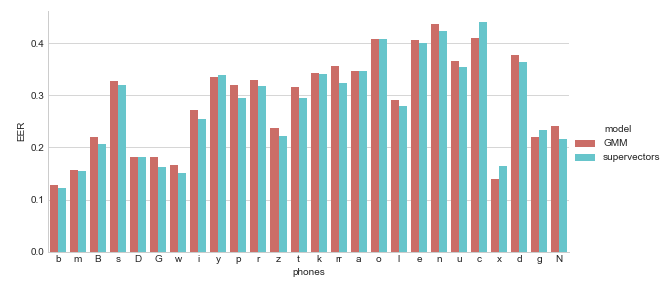
\includegraphics[width=0.8\textwidth]{files/figures/results/gmm-vs-supervectors/gmm-vs-supervectors-dev.png}
	\caption{Comparison of EER between Adapted GMMs
	and SVM trained on supervectors for all phones obtained in the development set, sorted
	in descending order according to their Kappa values.}
	\label{fig:gmmSupervectorsDev}
\end{figure}

At the end of the experimental phase,
the same experiment was carried out in the heldout set
leading to the results shown below
(Fig. \ref{fig:gmmSupervectorsTest}).
The models are trained using all the instances in the development set, namely, the
instances of the 4 folds.
They both have a very similar performance for each phone compared with the results obtained
in the development set (Fig. \ref{fig:gmmSupervectorsDev}),
from which one can deduce that both classifiers generalize well to
unobserved data. This time, however, it was the Adapted GMM model
which produced an overall weighted EER relative reduction of 0.8\% with respect to the SVMs
trained on supervectors. Even though the expected result would have been that the SVM performed
slightly better than the GMM, as it happened in the development set,
the degradation is less than 1\% so it is still a reasonable result.

\begin{figure}[H]
	\centering
	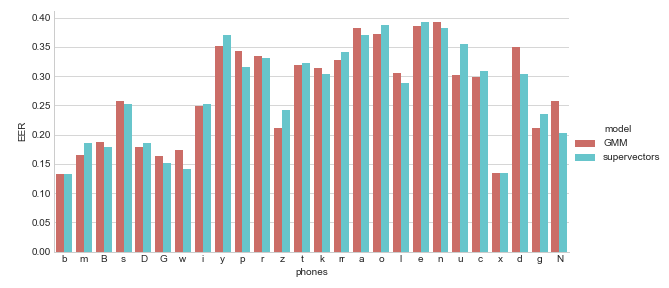
\includegraphics[width=0.8\textwidth]{files/figures/results/gmm-vs-supervectors/gmm-vs-supervectors-heldout.png}
	\caption{Comparison of EER between Adapted GMMs
	and SVM trained on supervectors for all phones obtained in the
	hold-out set, sorted in descending order according to their Kappa values.}
	\label{fig:gmmSupervectorsTest}
\end{figure}

After the successful replication of the initial experiments, a validated SVM model based on
supervectors is obtained. This classifier is used as baseline and starting point for
the next experiments.

\section{Tunning Experiments}

Tunning experiments are carried out in order to compare both alternative
dynamic features. Features are first analysed in isolation to
determine their best possible configurations.

After that, the features generated with those configurations are combined with
the supervectors and the results of those combinations are compared to each other.

Tunning is performed in the development set using 4-Fold Cross Validation. Results are
calculated only for the phones with high Kappa coefficients by averaging them.
Only these phones are considered in the process because they are the most reliable ones.

The most important parameter to be fitted is the number of coefficients to be used
for both methods. We assume this parameter to be phone-independent,
so it is shared
among all the phones. This helps to keep
the models simple by reducing the number of phone-dependent configuration parameters.

\subsection{Legendre Best System}

The objective of the Legendre tunning experiments is to find the optimum degree of the Legendre
Polynomials along with the best configuration.
Tunning the best Legendre features involves the analysis of
the following factors:

\begin{itemize}
	\item Legendre Polynomial degree
	\item Time axis normalization between -1 and 1
	\item Inclusion of duration
	\item Lasso-Regression regularization
\end{itemize}

Results are depicted in Fig. \ref{fig:legendreTunning}, which shows the variation of the
EER average taken over the phones with high Kappa
as function of the degree of the Legendre Polynomials for different configurations.
The analysis is restricted to polynomials up to degree 6 because
no further gains are obtained when using polynomials of higher degrees.

% An initial exploratory experiment showed that no further gains are obtained when using
% polynomials of degree higher than 6. Actually, results become worse when using many
% coefficients}.

\begin{figure}[H]
	\centering
	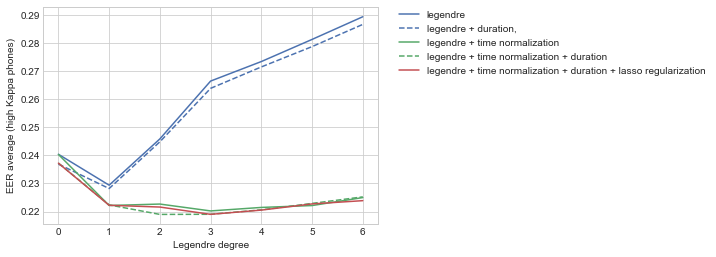
\includegraphics[width=1.0\textwidth]{files/figures/results/legendre-dct/legendre-tunning.png}
	\caption{EER average over phones with high Kappa for different
	degrees of Legendre Polynomials obtained in
	the development set. Additional configurations are also studied along with the degree and
	represented by different curves: time normalization, appending the duration and applying
	Lasso Regression.}
	\label{fig:legendreTunning}
\end{figure}

Time normalization before approximating the
MFCCs turns out to be an essential property for the Legendre Polynomials, evidenced by a
considerable reduction of the EER average (gap between the blue and green curves). At the same
time, appending the duration to the features produces a slight improvement in the performance.
Lasso Regularization, however, does not contribute to reduce the average EER.
Results show that the optimal configuration is to model the dynamics of the temporal dependencies
using Legendre Polynomials of degree 2,
along with normalizing the time axis and appending the duration of the
phone utterances to the features.

\subsection{DCT Best System and Comparison Between Features}

Analogous to Legendre, the objective of the DCT tunning experiments is to find the optimum
number of coefficients of DCT to approximate the dynamics of the temporal dependencies.
In the DCT case, the only additional parameter to be determined is whether or not appending the
duration to the DCT coefficients.

As in the Legendre optimal configuration, DCT tunning experiments also shows that appending the
duration to the coefficients produces a slight reduction in the averaged EER (around 1\%
relative).

A comparative plot between the variation of the EER as function of the number of coefficients
for both dynamic features is shown below in Fig. \ref{fig:legendreVsDCT}.
The additional parameters are fixed according to their optimal configuration
for both techinques:
Normalizing the time axis and appending the duration for Legendre (without Lasso Regularization),
and appending the duration for DCT. The degree of the Legendre Polynomials is mapped to
the number of coefficients in the \textit{x-axis} to allow the comparison:
the 0 degree Legendre Polynomial is mapped to 1 coefficient, the 1 degree Legendre Polynomial
is mapped to 2 coefficients, and so on.

\begin{figure}[H]
	\centering
	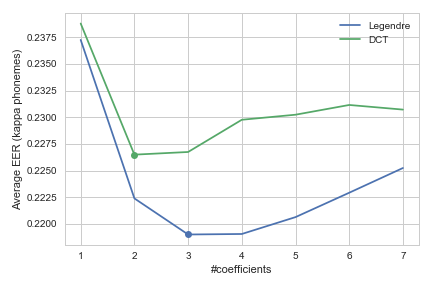
\includegraphics[width=0.5\textwidth]{files/figures/results/legendre-dct/legendre-dct-coefficients.png}
	\caption{EER average over phones with high Kappa as function of the number of coefficients
	for both Legendre Polynomials and DCT obtained in the development set.}
	\label{fig:legendreVsDCT}
\end{figure}

A dot is placed on each curve showing the optimal number of coefficients for both techniques.
As it is known from Fig. \ref{fig:legendreTunning},
the optimal number of coefficients for the
Legendre Polynomials is 3 (Polynomials of degree 2). Polynomials with 4 coefficients performs
almost as well as polynomials with 3 coefficients, but it is always preferable to keep the
model as simple as possible. On the other hand, the optimal number of coefficients for DCT is 2.

The results show that when the analysis is done in isolation (in absence of the supervectors
features), Legendre Polynomials lead to a better performance, generating a relative reduction
of the average EER of 3.3\% compared with DCT.

\subsection{Dynamic Features and Supervectors Combination Comparison}

Even though the SVM based solely on Legendre performs better than the SVM based solely on
DCT, a new experiment is carried out in order to determine which
dynamic feature integrates better
with the supervectors producing the best results. Two types of combination are
studied in the current thesis: a Features Combination and a Score
Combination.

In order to describe how the Features Combination is computed we recall some
concepts previously mentioned in the Method section.
As it is described in equation \ref{eq:svm}, a labeled set
\mbox{$D=\{ \ (x_{i}, y_{i}) \ | \ x_{i} \in \mathbb{R}^{p}, \ y_{i} \in \{-1, 1\} \ \}$}
is used
when training the SVM for a given phone, where $x_{i}$ represents the feature vector for the
$i^{th}$ instance of that phone and $y_{i}$ represents the label.
Let us denote:
\begin{equation}
	x_{i} =
	\begin{cases}
		s_{i} : [ \ s_{i1}, s_{i2}, \dotsc s_{in} \ ], & \text{when using supervectors features} \\
		d_{i} : [ \ d_{i1}, d_{i2}, \dotsc d_{im} \ ], & \text{when using dynamic features}
	\end{cases}
\end{equation}
Supervectors features are $n$-dimensional vectors while dynamic features are $m$-dimensional
vectors. When combining the features, dynamic features are appended to supervectors.
% (symbol ``$\circ$'' represents concatenation in Eq. \ref{eq:featuresCombination}).
A factor $c = \frac{n}{m}$ multiplies the dynamic features
in order to compensate the difference in
the number of features between supervectors and dynamic features.
Additionally, a weight factor $w \in \mathbb{R}$ that also multiplies the dynamic features
is chosen to determine
the priority, or importance \textit{a priori} of the dynamic features with respect to supervectors
within the SVM (the weight for supervectors is implicitly set to 1).
The higher the value of $w$, the less regularized are the dynamic features
at the beginning.
% The higher the value of $w$, the more relevant become the dynamic features.
The features combination vector for the $i^{th}$ instance is then computed as:
\begin{equation}
	x_{i}^{\prime} = s_{i} \circ (w * c * d_{i}) = [ \ s_{i1}, \ s_{i2}, \ \dotsc s_{in}, \ w * c * d_{i1}, \ w * c * d_{i2}, \ \dotsc w * c * d_{im} \ ]
	\label{eq:featuresCombination}
\end{equation}

where symbol ``$\circ$'' represents concatenation.

Score Combination, on the other hand, is computed by combining the scores
of the SVM classifiers trained independently on both supervectors and dynamic features.
Again, a weight $w \in \mathbb{R}$
is chosen to determine the amount of the score of the dynamic-feature-based system to be considered
in the final score. Let us denote
the score of the SVM trained on supervectors when classifying the $i^{th}$ instance
as $\text{sup}_{i}$ and the score of the SVM trained on dynamic features
when classifying the $i^{th}$ instance as
$\text{dyn}_{i}$.
% $\text{sup}_{i}$ to the score of the
% SVM trained on supervectors when classifing the $i^{th}$ instance,
% and $\text{dyn}_{i}$ to the score of the SVM trained on the dynamic features.

The final score for the
$i^{th}$ instance is computed as:
\begin{equation}
	\text{score}_{i} = \text{sup}_{i} + w * \text{dyn}_{i}
\end{equation}
The range of values to be explored for the parameter $w$ was adjusted empirically for both
Features Combination and Score Combination. The obtained interval to be explored for $w$ was
\mbox{[0.0 - 1.0]} with steps of 0.1. It is worth noting that choosing
a value for $w$ of 0.0 leads to not considering the dynamic features at all.

The experiment is again scoped to the phones with high Kappa values.
Weights to be used when combining the features and the scores are kept phone-dependent.
The objective is thus to compute two optimal weights for each phone:
one for the features combinations and the other one for the score combination.

% During the experiment, proportions of the dynamic features with respect to supervectors
% are varied between 0 and 1 with steps of 0.1.
% In other words, the explored interval is
% \mbox{[0.0, 0.1, 0.2 \ldots 1.0]}.
% 	An initial exploratory experiment showed that no further gains are obtained when using
% 	proportions higher than 1.0 for the dynamic features in neither features combination nor score combination
% 	experiments.
% It is worth noting that choosing
% a proportion of 0.0 of the dynamic
% features with respect to supervectors leads to not considering the dynamic features at all.

% both ends of the interval corresponds to use only
% a feature source and not using the other source at all. A proportion of 0.0 of the dynamic
% features with respect to supervectors leads to not considering the dynamic features at all
% while a proportion of 1.0 leads to not using the supervectors features at all.
% In the case of the Features Combination, an extra exploration is done in the interval
% [0.0 - 0.1], because achieving an optimal feature combination may have required a more
% refined granularity in the proportions. No significant gains, however, were observed
% when zooming in in the interval [0.0 - 0.1].

In the Features Combination experiment,
the optimal weight for the majority of the phones
for both Legendre and DCT approaches turns out to be 0.1.
% For the Features Combination case, the optimal proportion for the majority of the phonemes
% for both Legendre and DCT approaches is 0.1.
There are also some phones such as
$/\gamma/$ and $/b/$ for which the best weight is 0.0.
This can be interpreted as that
no weight produces an improvement when combining the dynamic features with the supervectors.

On the other hand, in the Score Combination experiment, the optimal weight for
the results of the different phones are more scattered along the whole interval [0.0 - 1.0]
for both Legendre and
DCT. Again, there are also some phones for which the optimal weight is 0.0, but they are
considerable fewer than in the features combination case.

For both combination types, the DCT features yield better results than the Legendre features,
though the results for both features are very close to each other (around 1\% of relative
difference), as it is shown in Table \ref{table:legendreVsDCTCombinations}.

~

\begin{table}[h]
	\renewcommand{\arraystretch}{1.5}
	\begin{center}
	    \begin{tabular}{ | c | c | c | }
	    \hline
	    & Legendre + Supervectors & DCT + Supervectors \\ \hline
	    EER Features Combination (Avg) & 0.188 & 0.187 \\ \hline
	    EER Score Combination (Avg) & 0.189  & 0.187 \\ \hline
	    \end{tabular}
	    \caption{EER average over phones with high Kappa using the best weight for
	    both Dynamic Features and combination approaches, obtained in the development set.}
	    \label{table:legendreVsDCTCombinations}
	\end{center}
\end{table}

At this point, the DCT features are chosen as the Dynamic Features to be combined with the
supervectors when training the final models, and for each of the remaining phones with
low Kappa values the phone-dependent weights are computed.

\textcolor{red}{
Even though training a system from the combination of the three features
(Supervectors, Legendre and DCT) was possible, it would have required the tunning of
an additional parameter for each phone, which is costly to mantain. Moreover, this
could have lead to overfitting the model. Because of these reasons, and the fact
that we weren't expecting significant gains in combining both types of dynamic features
because they model the same temporal characteristics,
we didn't explore a combination of the three features as a solution.
%the idea of combining the three features was discarded.
}

\section{Final Models Validation} \label{subsection:modelValidation}

The final experiments are carried out in order
to determine if there is a real gain when combining
supervectors with DCT features compared with training an SVM based only on supervectors.
Additionally, we are interested to see if any of both fusion systems is better
than the other one. The three systems to be compared are then:

\begin{itemize}
	\item SVM trained only on supervectors, which is used as the baseline system.
	\item SVM trained on the features combination of DCT and supervectors (using for each phone the best features combination weights obtained in the tunning phase).
	\item System based on the score combination of an SVM trained
	only on supervectors and an SVM trained
	only on DCT features (using for each phone the best score combination weights obtained in the tunning phase).
\end{itemize}

An initial experiment is performed in the development set
followed by a second experiment, where
the final models are tested against the heldout data.
The relative gains of the final models
are calculated using the SVM trained only on supervectors as baseline system.

Unlike the tunning phase, where the experimentation is driven by the results obtained
over the phones with higher kappa values, a new criteria is used for the model validation.
A McNemar's test is performed as previous step to scope the analysis
to a subset of phones with statistically significant gains in the development
data (\textit{p-value} $<$ 0.05).
McNemar's, which is described in Method Section \ref{subsection:mcnemar},
is used to estimate the confidence that a final model is different from
the baseline model by using the paired nominal results of both classifiers.

% McNemar is used to estimate confidence of the two classifiers being actually different
% using the paired nominal results of both classifiers (\ref{subsection:mcnemar}).
% The McNemar test is run using the SVM
% trained only on supervectors as baseline of the comparison.

\subsection{Development Results}

% The comparison of the three systems
% In order to make the comparison,
The three systems are trained applying 4-Fold Cross Validation
in the development set and then compared to each other.
% in the development set is carried out using the 4-Fold Cross Validation
% approach.
The EER for each of
the systems is computed
by gathering the scores from all the folds.
% obtained in each of the folds.
In addition, McNemar's test is also computed
over the scores from all the folds to determine if the
results yield statistically significant gains.

The phones for which the McNemar's test gives significant results
in the development set are:
% The results for all the phones are included in the tables
% (\ref{section:tables}) and plots (\ref{section:plots})
% of the Appendix. Rows with grey background corresponds to the phones for which
% the McNemar's test gives significant results in the development set, which are the
% phones of interest. Those are:

\begin{itemize}
	\item /s/, /y/, /e/, /o/, /l/, /n/, /m/ for Features Combination
	\item /s/, /y/, /e/, /o/, /l/, /z/, /n/, /m/, /rr/, /t/ for Score Combination
\end{itemize}

% The relative gains for the phones mentioned above are summarized in
The relative gains for those phones are summarized in
Fig. \ref{fig:fusionMcnemarDev} (results for all the phones are available
in tables \ref{section:tables} and plots \ref{section:plots} of the
Appendix). It is worth noting that phones that
give statistically significant gains in
the Score Combination experiment are a superset of the phones that give statistically
significant gains in the Features Combination experiment.
Three of the phones (/z/, /rr/, /t/) give statistically significant gains
when combining the scores but not when combining the features.
For that reason, only the bars associated with the Score Combination results are
included for those phones.

\begin{figure}[H]
	\centering
	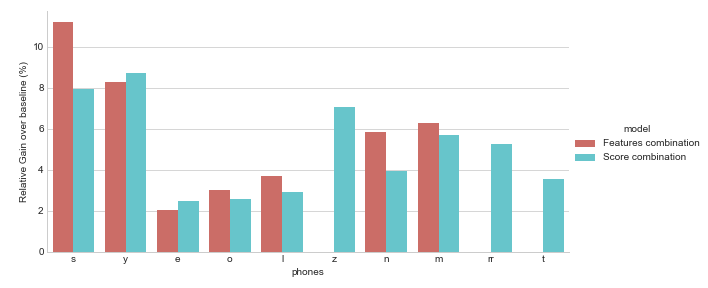
\includegraphics[width=0.8\textwidth]{files/figures/results/relatives/relatives-fusion-systems-dev-mcnemar.png}
	\caption{Comparison of relative gains over the Baseline systems
	between the Features Combination systems
	and the Score Combination systems
	computed on the development set.
	Results are sorted in descending order according to their McNemar's p-values.}
	\label{fig:fusionMcnemarDev}
\end{figure}

A Bootstrapping test is also performed in the development set to provide a complementary
analysis. As it is described in Method Section \ref{subsection:bootstrapping}, the main goal
is to compute the confidence intervals that enclose the 95\% of the samples of
the target distributions (in our case, EER distributions) to find out if they are shifted
with respect to each other. A thousand bootstrapping iterations are applied by resampling
the speakers and computing the EER over those speakers' instances.
Results are summarized in Fig. \ref{fig:bootstrappingDev}. Plots are split in two in order to adjust the y-axis and display the intervals
with greater detail.

The plots show that most of the fusion system intervals are shifted downwards with
respect to the supervectors-based baseline system,
which is a sign that fusion systems perform better than the
baseline systems.
% of a better performance in favor of the fusion systems.
% thus lowering the EER and leading
% to a better performance.
The only exception seems to be /z/, which
despite having almost identical confidence intervals for both systems,
it yields a significant difference
between the results obtained for the baseline system and the Score Combination system.
% A possible explanation for this is that the Score Combination system for the /z/
% phone is favored by the original distribution of the speakers in the development set.

\begin{figure}[H]
  \centering
  \begin{subfigure}{.47\textwidth}
    \centering
    \captionsetup{width=.95\linewidth}
    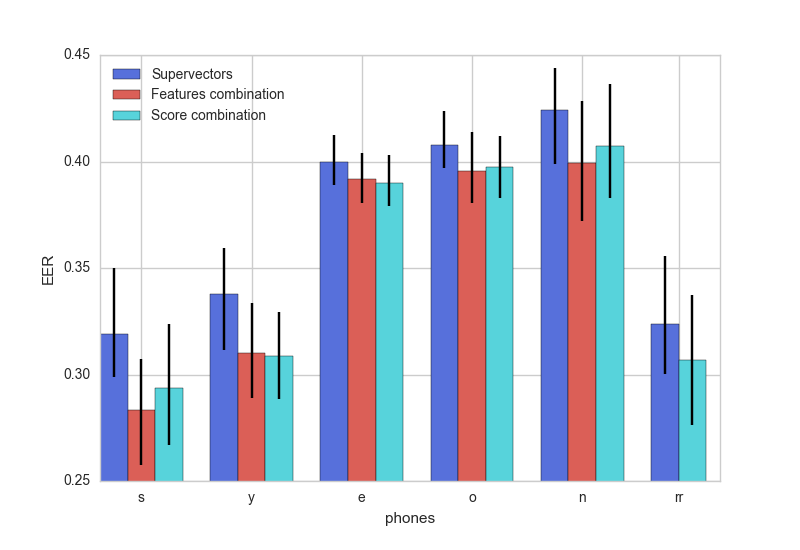
\includegraphics[width=1.08\linewidth, height=0.225\textheight]{files/figures/results/bootstrapping/bootstrapping_dev_2}
  \end{subfigure}
  \begin{subfigure}{.47\textwidth}
    \centering
    \captionsetup{width=.95\linewidth}
    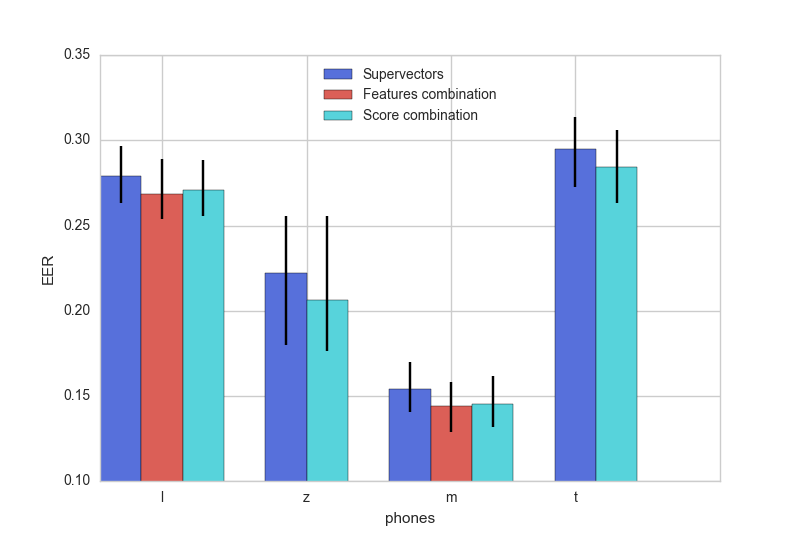
\includegraphics[width=.72\linewidth, height=0.225\textheight]{files/figures/results/bootstrapping/bootstrapping_dev_1}
  \end{subfigure}
  \caption{Comparison of 95\% confidence intervals for the baseline and fusion systems.
  A thousand iterations of Bootstrapping are applied
  in the development set for the phones that gave statistically significant gains in the
  McNemar's test.}
  \label{fig:bootstrappingDev}
\end{figure}

\subsection{Hold-out results}

In this experiment, the three aforementioned systems are trained using all the instances of the
development set and tested against the hold-out set.

The analysis is again scoped to our phones of interest, which are those with statistically
significant results in the development set.
The results for all the phones, however, are included in the tables
(\ref{section:tables}) and plots (\ref{section:plots})
of the Appendix.
Even though a new McNemar's test is computed on the
results obtained in the hold-out data, in many cases it does not yield statistically significant gains
for the phones of interest. This can be explained by the fact that hold-out data
has around 1/4 of the instances of the
development set, which results in very little testing data
affecting the efectiveness of the statistical test.

The relative gains for the phones of interest are summarized in Fig. \ref{fig:fusionMcnemarTest}.
Again, the bars for the three phones (/z/, /rr/, /t/) that gave statistically significant
gains when combining the scores but not when combininig the features in the development
set are only included for the Score Combination experiment.

\begin{figure}[H]
	\centering
	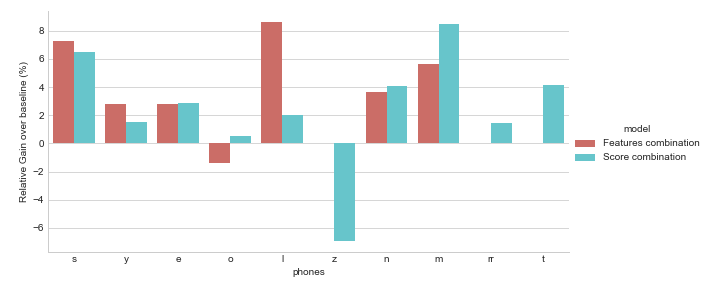
\includegraphics[width=0.9\textwidth]{files/figures/results/relatives/relative-fusion-systems-heldout-mcnemar.png}
	\caption{Comparison of relative gains over the Baseline systems
	between Features Combination systems and Score Combination
	systems computed on the hold-out set for the phones of interest.
	Results are sorted
	in descending order according to their McNemar's p-values computed on the development set.}
	\label{fig:fusionMcnemarTest}
\end{figure}

Results show that, for the phones that gave statistically significant gains
in the Score Combination
experiment carried out in the development set, only 'z' degrades its performance compared
with the baseline system (around a 6\% relative). Among the
remaining phones, some reduce its gain compared with the development set (such as
/y/ from 8\% to less than 2\% and /rr/ from almost 6\% to less than 2\%). Others such
as /m/ improves its gain from 6\% to more than 8\%.

On the other hand, results show that
for the phones that gave statistically significant gains in the
Features Combination experiment carried out in the development set, only /o/ degrades
its performance and only slightly.
Among the remaining phones, for the Features Combination experiment
there are cases where both improvements
and degradations of the performance are observed.

A Bootstrapping test is again performed in the hold-out set to provide a complementary analysis,
and the results are summarized in Fig. \ref{fig:bootstrappingHoldOut}.
The plots are again split in two in order to adjust the y-axis and display the intervals
with greater detail.

The most relevant thing to mention is that, unlike in the development set, the overlap
between the confidence intervals of the three systems is very big, to a point such that
for some phones it is difficult to determine if the intervals come from different
distributions. There are, though, some phones for which the intervals
for the fusion systems seem to be
shifted downwards with respect to the baseline system. The most representative example
is /s/, followed in lesser extent by other phones such as /l/, /m/, /t/, /e/ and /y/.

A positive aspect to be considered is that none of the phones degrade their
results in a significant manner. In addition,
the confidence intervals
for the two systems for the phone /z/ are very wide and they almost completely overlap,
which is an evidence that the degradation is not statistically significant.

% the overlap of the confidence intervals
% for the two systems for the phone /z/, which are very wide,
% Even the overlap for the confidence intervals for the phone /z/
% confidence itervals (which are very wide) for the phone /z/
% for both baseline and the score combination system overlap .
% which is a sign that \ldots

% At first glance, this may contradict the fact that
% performance of the Score Combination system for /z/ degrades 6\% with respect to the baseline
% system, as shown by the results show in Fig. \ref{fig:fusionMcnemarTest}.
% A possible explanation can be that the Score Combination system is not favored by
% the initial distribution of the speakers in the hold-out set, and is supported by
% the similarity of both intervals in Fig. \ref{fig:bootstrappingHoldOutB}.
% Additionally, in the results obtained in the development set (Fig. \ref{fig:bootstrappingDev}),
% there also was no evidence that one system was better than the other.

\begin{figure}[H]
  \centering
  \begin{subfigure}{.47\textwidth}
    \centering
    \captionsetup{width=.95\linewidth}
    % 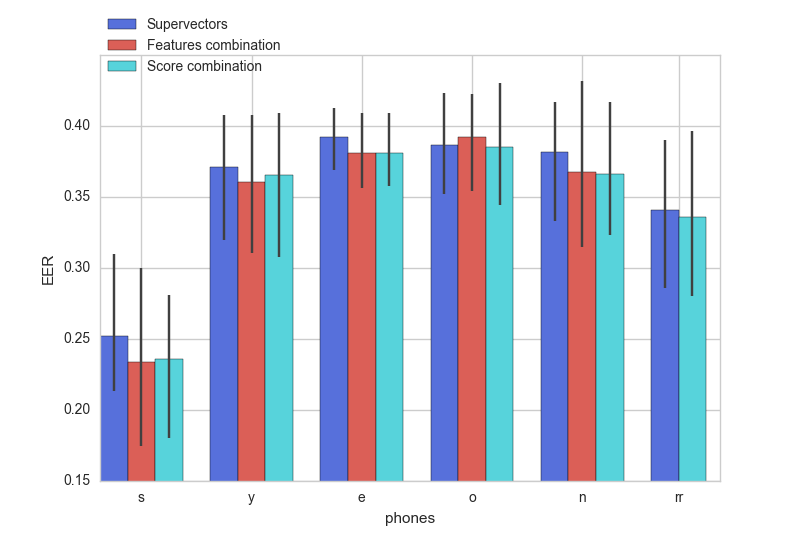
\includegraphics[width=.95\linewidth]{files/figures/results/bootstrapping/bootstrapping_heldout_2}
    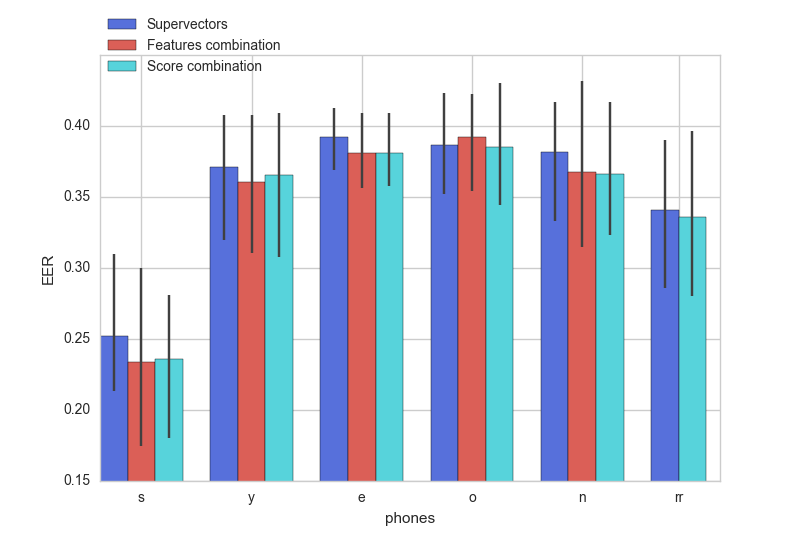
\includegraphics[width=1.08\linewidth, height=0.225\textheight]{files/figures/results/bootstrapping/bootstrapping_heldout_2}
    \caption{}
    \label{fig:bootstrappingHoldOutA}
  \end{subfigure}
  \begin{subfigure}{.47\textwidth}
    \centering
    \captionsetup{width=.95\linewidth}
    % 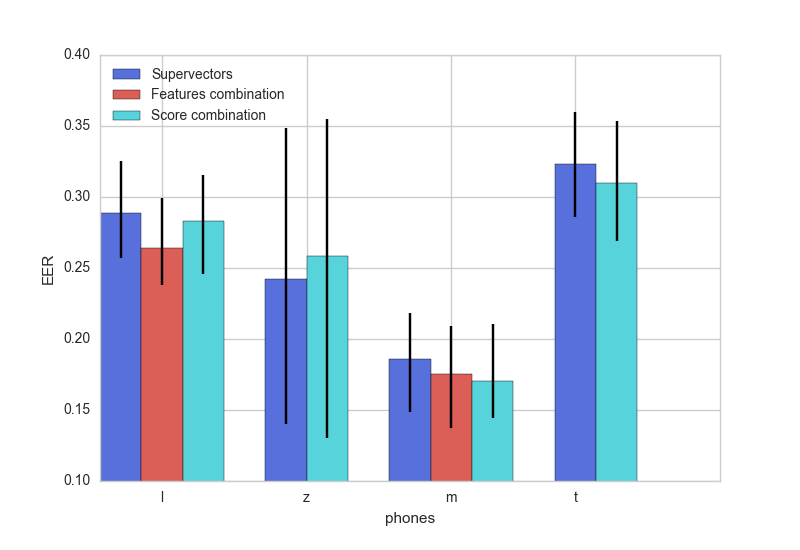
\includegraphics[width=.95\linewidth]{files/figures/results/bootstrapping/bootstrapping_heldout_1}
    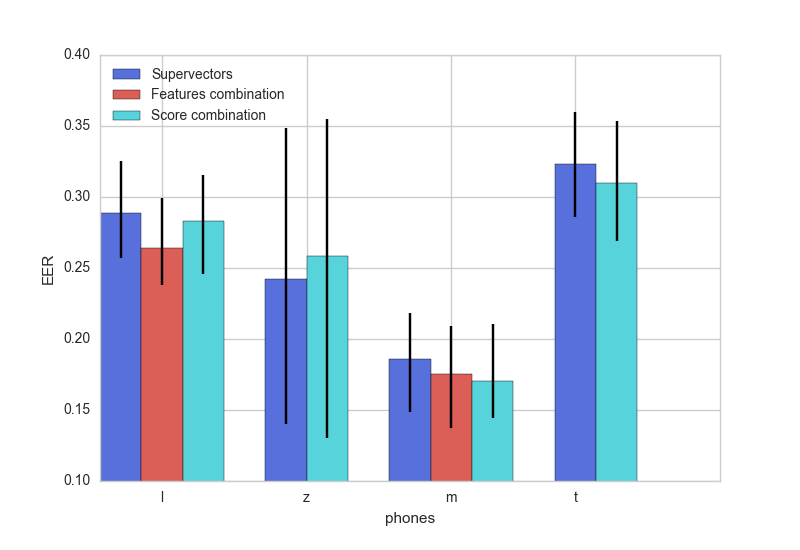
\includegraphics[width=.72\linewidth, height=0.225\textheight]{files/figures/results/bootstrapping/bootstrapping_heldout_1}
    \caption{}
    \label{fig:bootstrappingHoldOutB}
  \end{subfigure}
  \caption{Comparison of 95\% confidence intervals for the baseline and fusion systems.
  A thousand iterations of Bootstrapping are applied
  in the hold-out set for the phones of interest.}
  \label{fig:bootstrappingHoldOut}
\end{figure}


% One important aspect to be analysed in the next section is whether or not the Score Combination
% of the results leads to a more robust classifier than the Features Combination technique.


